\documentclass[conference]{IEEEtran}
\IEEEoverridecommandlockouts

\usepackage[spanish,es-tabla,es-nodecimaldot]{babel}
\usepackage[utf8]{inputenc}
\usepackage[T1]{fontenc}
\usepackage{cite}
\usepackage{amsmath,amssymb,amsfonts}
\usepackage{graphicx}
\usepackage{textcomp}
\usepackage{xcolor}
\usepackage{booktabs}
\usepackage{array}
\usepackage{tikz}
\usetikzlibrary{positioning,arrows.meta}
\usepackage{url}

% Nombres de clase en monoespaciada, como en el código.
\newcommand{\cls}[1]{\texttt{#1}}
\newcommand{\mb}{mala$\to$buena}

\begin{document}

\title{Clasificación de la calidad visual de frutas y verduras con imágenes: modelos clásicos, CNN y evaluación sin fuga entre grupos}

\author{
\IEEEauthorblockN{Ismael Barrionuevo}
\IEEEauthorblockA{\textit{Universidad Icesi}\\Cali, Colombia}
\and
\IEEEauthorblockN{David Chicué}
\IEEEauthorblockA{\textit{Universidad Icesi}\\Cali, Colombia}
\and
\IEEEauthorblockN{Daniel Martinez}
\IEEEauthorblockA{\textit{Universidad Icesi}\\Cali, Colombia}
}

\maketitle

\begin{abstract}
Presentamos un prototipo que, a partir de la foto de una sola pieza sobre fondo sencillo, identifica el producto (13 frutas y verduras), clasifica su apariencia externa como buena, regular o mala y estima su tamaño relativo en el encuadre. Integramos tres conjuntos públicos (Kaggle/FruitNet, AgriFreshNET y AFruitDB), fotos propias y fotos de celular aportadas por el curso. Segmentamos la pieza con OpenCV, extraemos 359 atributos de color, textura y forma, y comparamos regresión logística, SVM lineal, Random Forest y una CNN de cuatro bloques entrenada desde cero. La decisión metodológica central es partir los datos por grupos de captura (ráfagas, semanas de fotos de un mismo lote y sesiones): sin ella, el F1 de Kaggle se inflaba unos 3,5 puntos. Los hiperparámetros se eligen con validación cruzada agrupada, y validación y prueba se usan una sola vez. El modelo final, un Random Forest elegido en validación por cometer menos errores ``mala predicha como buena'', obtiene en prueba un F1 macro de 0,596 (IC 95\,\% por grupos: 0,522--0,677), deja pasar 40 de 1502 piezas malas como buenas y acierta el producto en el 79,5\,\% de las fotos. En la prueba externa con fotos de celular el desempeño cae (F1 0,295) y solo se reconocen las frutas que tuvieron fotos de celular en el entrenamiento, lo que delimita con claridad para qué sirve el sistema.
\end{abstract}

\begin{IEEEkeywords}
calidad de frutas, visión por computadora, Random Forest, red neuronal convolucional, fuga de datos, validación agrupada, CRISP-DM
\end{IEEEkeywords}

\section{Introducción}

En plazas de mercado y tiendas, la calidad de frutas y verduras se juzga a simple vista. El resultado depende de la experiencia de quien mira y de la luz, y una pieza deteriorada que se vende como buena afecta al comprador y a la confianza en el vendedor. Una revisión asistida por visión por computadora puede dar una primera opinión consistente, siempre que se diga con honestidad cuándo funciona y cuándo no.

El problema tiene tres salidas: \emph{qué} producto es, \emph{en qué estado} está su apariencia externa (buena, regular o mala) y \emph{qué tan grande} se ve en la foto. Los errores no cuestan lo mismo: predecir \cls{bad} como \cls{good} (en adelante, \emph{\mb}) es el más caro, porque deja pasar producto deteriorado; descartar una pieza buena es desperdicio, pero no un riesgo para el consumidor.

Seguimos la metodología CRISP-DM~\cite{chapman2000}. Las contribuciones son: (i) un pipeline reproducible, con un comando por paso, que va de las fotos crudas a una app de Streamlit; (ii) una partición por grupos de captura que elimina una fuga real y medida; (iii) la comparación de cuatro modelos bajo un mismo protocolo, con la elección del modelo final guiada por el costo asimétrico de los errores; y (iv) una prueba externa con fotos de celular, etiquetadas a ciegas, que mide el cambio de dominio. El código, los resultados y los notebooks están en el repositorio del proyecto\footnote{\url{https://github.com/Davinerto9/fruit-vegetable-quality-classifier-ml}}, y la presentación del proyecto está en video\footnote{\url{https://youtu.be/gwlolsmqH44}}.

\section{Fundamentos teóricos}

\subsection{Formulación del problema}

Sea $\mathcal{D}=\{(x_i,y_i,p_i,s_i,g_i)\}_{i=1}^{N}$ el conjunto de datos. Cada foto RGB es $x_i\in\{0,\dots,255\}^{H_i\times W_i\times 3}$; $y_i\in\mathcal{Y}=\{\cls{good},\cls{regular},\cls{bad}\}$ la calidad visible, $p_i$ el producto (13 clases), $s_i$ la fuente y $g_i$ el grupo de captura. $s_i$ y $g_i$ no son entradas del modelo: sirven para particionar y auditar. El sistema es una composición de funciones sobre la misma segmentación $S$:
\begin{equation}
\hat y=h_\theta\big(\phi(S(x))\big),\quad
\hat p=f_\psi\big(\phi(S(x))\big),\quad
\hat t=\tau\big(d_n(S(x))\big),
\label{eq:sistema}
\end{equation}
donde $S(x)=(c,m)$ es un recorte $c\in\mathbb{R}^{128\times128\times3}$ con su máscara binaria $m$; $\phi$ extrae 359 atributos (para la CNN, $\phi(c,m)=c\odot m$); $h_\theta$ y $f_\psi$ son clasificadores; y $\tau$ convierte el diámetro normalizado $d_n$ en pequeño/mediano/grande.

Con una matriz de costos $C_{jk}$ (costo de predecir $k$ si la clase real es $j$), el objetivo ideal es minimizar el riesgo $R(h)=\mathbb{E}_{(x,y)}[C_{y,h(x)}]$, con $C_{\text{bad},\text{good}}$ como el mayor. Como $C$ no se conoce con precisión, se entrena con un sustituto, la entropía cruzada ponderada
\begin{equation}
L(\theta)=-\frac{1}{N}\sum_i \omega_{y_i}\log p_\theta(y_i\mid x_i),\qquad
\omega_k=\frac{N}{K N_k},
\label{eq:perdida}
\end{equation}
que hace que cada clase aporte lo mismo a la pérdida, y se reporta aparte el número de errores \mb. Finalmente, lo que interesa es el error sobre \emph{capturas nuevas}, no sobre fotos casi idénticas a las de entrenamiento; por eso cada grupo $g$ debe quedar completo en una sola partición (Sec.~\ref{sec:particion}).

\emph{Por qué es un problema complejo.} (1) La entrada es de alta dimensión y la señal útil (una mancha) ocupa una fracción pequeña. (2) Las etiquetas son heterogéneas: cada fuente usa su propia escala, y el mapeo a $\mathcal{Y}$ es una decisión de modelado. (3) Fuente y clase están confundidas: en el inventario, el 82\,\% de las fotos \cls{regular} vienen de AgriFreshNET. (4) Las observaciones no son independientes: hay ráfagas, aumentos y semanas de fotos de las mismas piezas. (5) El tamaño real no es identificable sin escala (Sec.~\ref{sec:preparacion}).

\subsection{Segmentación}

La foto se reduce a 320\,px de lado mayor y se pasa a CIE Lab, donde las sombras cambian sobre todo $L$ y no la cromaticidad $(a,b)$. Con k-means ($k=3$) sobre una franja del borde se estiman los colores del fondo $\{\mu_j\}$, y cada píxel recibe $\mathrm{score}(u)=\min_j\lVert(a_u,b_u)-(a_j,b_j)\rVert_2$ más un término que recupera zonas muy oscuras (podredumbre). El umbral se elige con Otsu~\cite{otsu1979}, que maximiza la varianza entre clases $\omega_0\omega_1(\mu_0-\mu_1)^2$. La máscara se refina con GrabCut~\cite{rother2004}, que minimiza una energía de campo aleatorio de Markov mediante cortes de grafo. Una transformada de distancia y \emph{watershed} cuentan las piezas: si hay más de una, si la foto está en escala de grises o si la máscara es implausible, la foto se rechaza en lugar de clasificarse.

\subsection{Atributos y modelos clásicos}

Sobre los píxeles $\Omega$ de la máscara se calculan (i) histogramas normalizados de 16 bins en R, G, B, H, S y V (96 atributos), invariantes al tamaño de la pieza; (ii) el histograma de patrones binarios locales, LBP~\cite{ojala2002}, $\mathrm{LBP}(u)=\sum_{k=0}^{7}\mathbf{1}[I(v_k)\ge I(u)]\,2^k$ (256 atributos), invariante a cambios monótonos de brillo y sensible a arrugas y moho; y (iii) siete descriptores de forma, como la circularidad $4\pi A/P^2$ y la elongación $\sqrt{\lambda_2/\lambda_1}$. En total, 359 atributos.

La \emph{regresión logística} multinomial (línea base) modela $P(y=k\mid z)=\mathrm{softmax}_k(w_k^\top z+b_k)$ y es convexa. La \emph{SVM lineal}~\cite{cortes1995} maximiza el margen $2/\lVert w\rVert$ con pérdida bisagra al cuadrado, uno contra el resto. Ambas usan atributos estandarizados con media y desviación estimadas solo en entrenamiento. El \emph{Random Forest}~\cite{breiman2001} promedia $T$ árboles que eligen cortes por reducción de la impureza de Gini $G=1-\sum_k\hat p_k^2$, cada uno con una muestra \emph{bootstrap} y $m$ atributos al azar por nodo. Si cada árbol tiene varianza $\sigma^2$ y correlación $\rho$, la varianza del promedio es $\rho\sigma^2+(1-\rho)\sigma^2/T$: el submuestreo baja $\rho$ y promediar elimina el segundo término.

\subsection{Red convolucional}

La CNN recibe $c\odot m$ en $[0,1]$ y apila cuatro bloques Conv\,3$\times$3 $\to$ BatchNorm~\cite{ioffe2015} $\to$ ReLU $\to$ MaxPool\,2$\times$2 con 32, 64, 128 y 256 filtros, seguidos de \emph{global average pooling}, \emph{dropout} ($p=0{,}35$) y softmax: 389\,667 parámetros. Con $r_\ell=r_{\ell-1}+(k-1)j_{\ell-1}$, el campo receptivo del último bloque es de 46$\times$46\,px (36\,\% del recorte), suficiente para abarcar una lesión con su contexto; con tres bloques era de 22\,px. Se optimiza con Adam~\cite{kingma2015}.

\subsection{Métricas e incertidumbre}

Con $P_k$ y $R_k$ la precisión y el recall de la clase $k$, $\mathrm{F1}_{\text{macro}}=\frac{1}{K}\sum_k 2P_kR_k/(P_k+R_k)$, que pesa igual a \cls{regular} aunque sea minoritaria. Como las fotos de un grupo están correlacionadas, los intervalos del 95\,\% se calculan con \emph{bootstrap} por grupos~\cite{efron1993}: se remuestrean grupos completos con reemplazo y se toman los percentiles 2,5 y 97,5. Para comparar dos modelos se usa el \emph{bootstrap} pareado de la diferencia $\Delta$ sobre las mismas réplicas.

\begin{figure}[t]
\centering
\begin{tikzpicture}[
  box/.style={draw, rounded corners=1pt, align=center, font=\scriptsize,
              text width=17mm, minimum height=9.5mm, inner sep=1pt},
  arr/.style={-{Stealth[length=1.6mm]}, thin}]
% Rejilla fija: 4 columnas separadas 2,2 cm y 2 filas separadas 1,4 cm.
\node[box] (inv) at (0,0)       {Inventario\\fuente, grupo};
\node[box] (seg) at (2.2,0)    {Segmentación\\recorte 128$\times$128};
\node[box] (par) at (4.4,0)     {Partición\\por grupos};
\node[box] (att) at (6.6,0)    {359\\atributos};
\node[box] (app) at (0,-1.4)    {App\\Streamlit};
\node[box] (ev)  at (2.2,-1.4) {Val, test y celular (1 vez)};
\node[box] (cnn) at (4.4,-1.4)  {CNN\\4 bloques};
\node[box] (cls) at (6.6,-1.4) {LR, SVM, RF\\(GridSearch)};
\draw[arr] (inv) -- (seg);
\draw[arr] (seg) -- (par);
\draw[arr] (par) -- (att);
\draw[arr] (att) -- (cls);
\draw[arr] (par) -- (cnn);
\draw[arr] (cls) -- (cnn);
\draw[arr] (cnn) -- (ev);
\draw[arr] (ev)  -- (app);
\end{tikzpicture}
\caption{Flujo del sistema. Los modelos solo ven \emph{train}; validación, prueba y fotos de celular se evalúan una vez cada una, y la app reutiliza la misma segmentación y los mismos atributos.}
\label{fig:flujo}
\end{figure}

\begin{table}[t]
\caption{Fuentes de datos (archivos con etiqueta de calidad)}
\label{tab:fuentes}
\centering
\scriptsize
\setlength{\tabcolsep}{1.8pt}
\begin{tabular}{@{}lccccc@{}}
\toprule
Fuente & buena & regular & mala & Grupos & Licencia\\
\midrule
Kaggle / FruitNet \cite{meshram2022,park_kaggle} & 11\,664 & 0 & 6\,788 & 834 & CC0\\
AgriFreshNET \cite{risdin2026} & 4\,677 & 4\,695 & 4\,720 & 177$^a$ & CC BY 4.0\\
AFruitDB \cite{mojumdar2024data} & 929 & 1\,035 & 394 & 39 & CC BY 4.0\\
Propias & 24 & 15 & 2 & 7 & ---\\
Celular, mitad de prueba \cite{apo3_fotos} & 250 & 48 & 4 & 6 & ---\\
\bottomrule
\multicolumn{6}{@{}p{0.95\columnwidth}}{$^a$ producto $\times$ semana, tras unir las fotos de un mismo lote (Sec.~\ref{sec:particion}).}
\end{tabular}
\end{table}

\section{Metodología}

La Fig.~\ref{fig:flujo} resume el flujo. Cada paso es un comando (\texttt{python -m src.main <paso>}) que lee lo que dejó el anterior, con semilla 42 en todo lo aleatorio.

\subsection{Datos}

La Tabla~\ref{tab:fuentes} resume las fuentes. Las clases de cada una se mapearon a $\mathcal{Y}$: Good/Bad de Kaggle~\cite{park_kaggle}, redistribución de FruitNet~\cite{meshram2022}; Fresh/Semi-Fresh/Rotten de AgriFreshNET~\cite{risdin2026}; y los grados 1st/2nd/3rd de AFruitDB~\cite{mojumdar2025,mojumdar2024data}, que agregamos para que \cls{regular} no dependiera de una sola fuente y que aporta el mango. Las 1074 fotos \emph{Mixed} de Kaggle, con varias piezas de calidades distintas, no tienen etiqueta por pieza y no se usan. Los grupos de AgriFreshNET en los que una misma imagen aparece con dos etiquetas (18 grupos, 247 archivos) se excluyen. Las fotos propias (42, de las cuales 41 tienen estado: la restante es un racimo que requiere etiqueta por pieza) y las del pool de celular del curso~\cite{apo3_fotos} se etiquetaron con los criterios visuales documentados en el repositorio.

El análisis exploratorio mostró tres rasgos que condicionan todo lo demás. Primero, el desbalance (49\,\% buena, 16\,\% regular y 34\,\% mala en archivos). Segundo, casi cada producto viene de una sola fuente, y cada fuente tiene su propio fondo, resolución (mediana de 256\,px en Kaggle, 512\,px en AgriFreshNET y 4000\,px en AFruitDB) y nitidez. Tercero, la dependencia entre fotos: los grupos de Kaggle tienen en mediana 10 fotos y los de AFruitDB 29.

\subsection{Preparación y tamaño}
\label{sec:preparacion}

De 34\,943 fotos etiquetadas, la segmentación marcó 26\,015 recortes como candidatos; tras apartar los grupos en conflicto y los excluidos en la revisión visual, y sumar la mitad de entrenamiento del celular, el reparto final usa 25\,973. Kaggle es la fuente con más rechazos (36\,\% a revisión, sobre todo por tener dos o más frutas, y las 1188 en escala de grises, todas de la clase buena, que serían un atajo). Con el área $A$ de la máscara se calcula $d_n=2\sqrt{A/\pi}/\max(H,W)$. Por el modelo de cámara estenopeica, $d_n\approx\frac{f}{\max(H,W)}\frac{D}{Z}$: depende del cociente entre diámetro real $D$ y distancia $Z$, así que sin una referencia de escala \emph{el tamaño real no es identificable}. Los umbrales (pequeño $<0{,}33\le$ mediano $<0{,}55\le$ grande) se calibraron con 35 fotos propias y coinciden con 34; solo hay dos ejemplos pequeños y ninguno grande, por lo que se reporta como ocupación relativa del encuadre y no como centímetros.

\subsection{Partición por grupos}
\label{sec:particion}

Cada grupo se asigna completo a \emph{train}, validación o prueba (objetivo 70/15/15). Entre 4096 permutaciones aleatorias de los grupos se elige la que no deja clases ni productos ausentes y minimiza el error cuadrático ponderado de proporciones por estrato. La definición correcta de grupo se encontró en tres intentos sobre los mismos recortes: (1) una foto con sus aumentos, pero el 99\,\% de las fotos de Kaggle en validación tenía una ``gemela'' de la misma ráfaga en \emph{train}, y el F1 de Kaggle subía de 0,932 a 0,968; (2) además, las ráfagas de Kaggle por fecha y minuto, pero AgriFreshNET seguía fotografiando las mismas piezas durante semanas (en validación, 727 grupos eran en realidad 82 semanas); y (3) además, producto y semana en AgriFreshNET, y sesión en AFruitDB y en las fotos de celular. Así, los 5188 grupos iniciales de AgriFreshNET se convierten en 177. El reparto final tiene 18\,199 recortes en \emph{train} (incluida la mitad de entrenamiento de las fotos de celular), 3605 en validación (129 grupos) y 4169 en prueba (184 grupos). Este es el tipo de fuga que Kapoor y Narayanan~\cite{kapoor2023} señalan como una causa frecuente de resultados inflados.

\subsection{Modelos y ajuste de hiperparámetros}

Los modelos clásicos se ajustan con \texttt{GridSearchCV} de scikit-learn~\cite{pedregosa2011}, con \texttt{StratifiedGroupKFold(3)} sobre \emph{train} y F1 macro como criterio; el mejor se reentrena con todo \emph{train} (Tabla~\ref{tab:rejillas}). Los pesos de clase $\omega_k$ se calculan solo con \emph{train}. Para la CNN no hay validación cruzada (una hora por entrenamiento en CPU): la arquitectura viene de experimentos del segundo reparto (tres bloques subajustaban; los giros como aumento de datos bajaron el F1 en 0,051), y la parada temprana (paciencia 12) y la reducción del \emph{learning rate} usan un 10\,\% de los grupos de \emph{train}, no la validación. El estado final candidato del ensamble promedia $\hat p=0{,}5\,p_{\text{RF}}+0{,}5\,p_{\text{CNN}}$, con el peso fijado antes de evaluar.

\emph{Alternativas descartadas.} KNN, porque en 359 dimensiones las distancias se concentran y predecir cuesta $O(n)$ por foto. Un árbol único, por su varianza alta; el RF es su versión promediada. La SVM con kernel RBF, cuyo entrenamiento crece de forma superlineal con más de 16\,000 muestras. XGBoost, que podría mejorar al RF pero agrega muchos hiperparámetros que se elegirían sobre los mismos datos. El \emph{transfer learning} (MobileNet, ResNet), porque la consigna prioriza modelos entrenados desde cero; queda como cota superior en trabajo futuro. Los giros como aumento de datos se probaron y se descartaron ($-0{,}051$ de F1). Ajustar el peso del ensamble en validación habría sido seleccionar con validación. Predecir el tamaño en centímetros no es posible sin una referencia de escala (Sec.~\ref{sec:preparacion}).

\begin{table}[t]
\caption{Rejillas de búsqueda y configuración elegida por la validación cruzada agrupada}
\label{tab:rejillas}
\centering
\scriptsize
\setlength{\tabcolsep}{2pt}
\begin{tabular}{@{}lll@{}}
\toprule
Modelo & Rejilla & Elegido\\
\midrule
Logística & $C\in\{0{,}1;1;10\}$ & $C=0{,}1$\\
SVM lineal & $C\in\{0{,}1;1;10\}$ & $C=0{,}1$\\
RF estado & hoja $\in\{1,5,20\}$; profundidad & hoja 20, sin límite,\\
($T=200$) & $\in\{\infty,20\}$; $m\in\{\sqrt{p},0{,}1p\}$ & $m=0{,}1p$\\
RF producto & hoja $\in\{1,5\}$; $m\in\{\sqrt{p},0{,}1p\}$ & hoja 1, $m=0{,}1p$\\
CNN & 4 bloques; Adam, $\eta_0=10^{-3}$; lote 64 & mejor época: 18/30\\
\bottomrule
\end{tabular}
\end{table}

\begin{table}[t]
\caption{Estado: F1 macro por modelo y errores \mb}
\label{tab:estado}
\centering
\scriptsize
\setlength{\tabcolsep}{4pt}
\begin{tabular}{@{}lccccc@{}}
\toprule
 & \multicolumn{2}{c}{Validación} & \multicolumn{3}{c}{Prueba}\\
\cmidrule(lr){2-3}\cmidrule(l){4-6}
Modelo & F1 & M$\to$B & F1 & M$\to$B & Rec.\ mala\\
\midrule
Reg.\ logística & 0,706 & 124 & 0,560 & 86 & 0,782\\
SVM lineal & 0,699 & 122 & 0,566 & 80 & 0,815\\
CNN & 0,738 & 120 & 0,603 & 190 & 0,771\\
Ensamble & 0,769 & 82 & 0,621 & 101 & 0,832\\
\textbf{RF (final)} & \textbf{0,762} & \textbf{41} & \textbf{0,596} & \textbf{40} & \textbf{0,871}\\
\bottomrule
\multicolumn{6}{@{}l}{M$\to$B: malas predichas como buenas. Val: 3605 fotos; prueba: 4169.}\\
\multicolumn{6}{@{}l}{IC 95\,\% del RF: val [0,697; 0,850]; prueba [0,522; 0,677].}\\
\multicolumn{6}{@{}l}{Producto (RF, 13 clases): accuracy 86,9\,\% (val) y 79,5\,\% (prueba).}
\end{tabular}
\end{table}

\subsection{Protocolo de evaluación}

La validación y la prueba no eligen nada y se usan una vez. Antes de la prueba, \texttt{congelar} guarda la huella SHA-256 de la partición y de los cinco modelos; la evaluación de prueba verifica esa huella y crea un candado que impide repetirla. La elección del modelo final se registró en el repositorio antes de abrir la prueba. Las fotos de celular del curso se partieron \emph{por sesión} en dos mitades antes de etiquetarlas: una se suma a \emph{train} y la otra es una prueba externa, etiquetada a ciegas (sin ver la app) y evaluada una vez. Se reportan F1 macro, la matriz de confusión, el recall de \cls{bad}, los errores \mb{} y el F1 por fuente, porque Kaggle solo tiene dos clases.

\subsection{Despliegue}

La app de Streamlit recibe una foto cargada o de la cámara, reutiliza las funciones de \texttt{src/} (una prueba automática verifica que los atributos calculados en memoria coinciden valor por valor con los del entrenamiento) y muestra el producto, el estado con sus probabilidades, el contorno detectado y $d_n$. Si la probabilidad del producto es menor que 0,5, responde que no lo reconoce; si la foto tiene varias piezas o la máscara es dudosa, pide otra foto. Las imágenes se procesan en memoria y no se guardan.

\section{Resultados}

La Tabla~\ref{tab:estado} y la Fig.~\ref{fig:f1} comparan los modelos de estado. En validación, Random Forest, CNN y ensamble empatan en F1: las diferencias pareadas frente a RF incluyen el cero (ensamble $-$ RF: $+0{,}007$ $[-0{,}043;+0{,}049]$). En cambio, el RF deja pasar significativamente menos piezas malas como buenas (ensamble $-$ RF: $+41$ $[+9;+80]$; CNN $-$ RF: $+79$ $[+24;+140]$). Por eso, y antes de abrir la prueba, se eligió el RF como modelo final.

En la prueba, el RF obtiene un F1 de 0,596 y comete 40 errores \mb{} (2,7\,\% de las malas). El ensamble obtiene algo más de F1 (0,621), pero la diferencia no es significativa ($+0{,}025$ $[-0{,}030;+0{,}093]$), mientras que deja pasar 61 malas más $[+23;+107]$. El criterio de costo se sostiene fuera de muestra. La Fig.~\ref{fig:confusion} muestra dónde falla el RF: casi toda la pérdida está en \cls{regular}, con un recall de 0,26.

\begin{figure}[t]
\centering
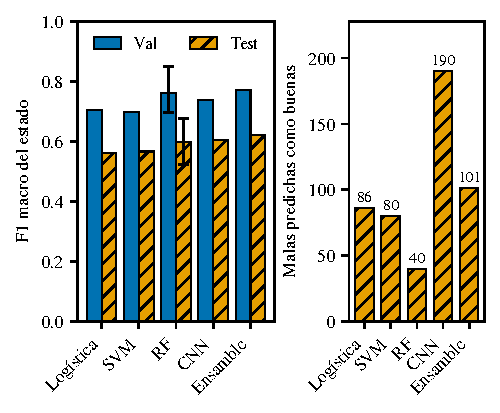
\includegraphics[width=\columnwidth]{figuras/f1_y_errores.pdf}
\caption{Izquierda: F1 macro del estado (RF: Random Forest) en validación y prueba, con el IC 95\,\% por grupos del modelo final. Derecha: piezas malas predichas como buenas en prueba (1502 malas en total).}
\label{fig:f1}
\end{figure}

\begin{figure}[t]
\centering
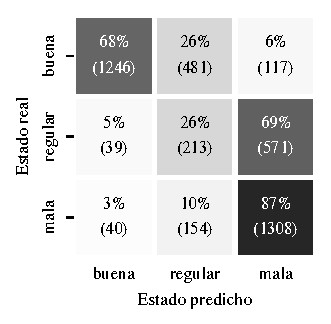
\includegraphics[width=0.72\columnwidth]{figuras/confusion_rf_test.pdf}
\caption{Matriz de confusión del Random Forest en prueba, normalizada por fila (entre paréntesis, el número de fotos).}
\label{fig:confusion}
\end{figure}

Por fuente (Tabla~\ref{tab:fuente}), el problema binario de Kaggle se resuelve bien (0,93), mientras que las cifras representativas de tres clases son las de AgriFreshNET y AFruitDB. AFruitDB tiene en prueba solo 178 fotos de 6 sesiones, así que su cifra es poco estable.

En la prueba externa con fotos de celular (302 fotos, 6 sesiones; 250 buenas, 48 regulares y 4 malas), el RF obtiene un F1 de 0,295 $[0{,}227;0{,}334]$ y acierta el producto en el 31,8\,\% de las fotos [5,3\,\%; 76,4\,\%]. Por fruta (Tabla~\ref{tab:celular}), el resultado se divide en dos: las que tuvieron fotos de celular en la mitad de entrenamiento se reconocen, y las demás casi nunca.

\begin{table}[t]
\caption{F1 macro del estado por fuente (Random Forest)}
\label{tab:fuente}
\centering
\scriptsize
\begin{tabular}{@{}lccc@{}}
\toprule
Partición & Kaggle (2 clases) & AgriFreshNET & AFruitDB\\
\midrule
Validación & 0,966 & 0,661 & 0,655\\
Prueba & 0,932 & 0,431 & 0,613\\
\bottomrule
\end{tabular}
\end{table}

\begin{table}[t]
\caption{Prueba externa con fotos de celular: acierto del producto}
\label{tab:celular}
\centering
\scriptsize
\begin{tabular}{@{}lccc@{}}
\toprule
Fruta & Fotos & Acierto & ¿Celular en \emph{train}?\\
\midrule
Banano & 18 & 100\,\% & sí\\
Manzana & 35 & 89\,\% & sí\\
Naranja & 49 & 94\,\% & no\\
Guayaba & 91 & 1\,\% & no\\
Limón & 70 & 0\,\% & no\\
Mango & 39 & 0\,\% & no\\
\bottomrule
\end{tabular}
\end{table}

\section{Análisis de resultados}

\emph{Sesgo, varianza y sobreajuste.} Los modelos lineales tienen F1 de 0,77 en \emph{train}, 0,57--0,59 en la validación cruzada agrupada y 0,70--0,71 en validación; la CV eligió la regularización más fuerte ($C=0{,}1$), y el techo de la frontera lineal explica que queden por debajo de los no lineales. El RF llega a 0,93 en \emph{train} y 0,60 en la CV: los árboles memorizan, y que la CV elija las hojas más grandes de la rejilla (20 muestras) confirma que hacía falta regularizar. En la CNN (Fig.~\ref{fig:perdida}), la pérdida de \emph{train} sigue bajando hasta la época 30 (0,15), mientras que la del holdout toca su mínimo en la época 18 (0,355, con accuracy 0,883 frente a 0,903 en \emph{train}) y luego oscila: hay sobreajuste, contenido por la parada temprana, que restaura los pesos de la mejor época. En el segundo reparto, la secuencia tres bloques $\to$ tres bloques con giros $\to$ cuatro bloques funcionó como experimento del dilema sesgo--varianza: con tres bloques, \emph{train} y validación estaban juntos y con pérdida alta (sesgo); regularizar con giros empeoró; y aumentar la capacidad (campo receptivo de 22 a 46\,px) mejoró.

\begin{figure}[t]
\centering
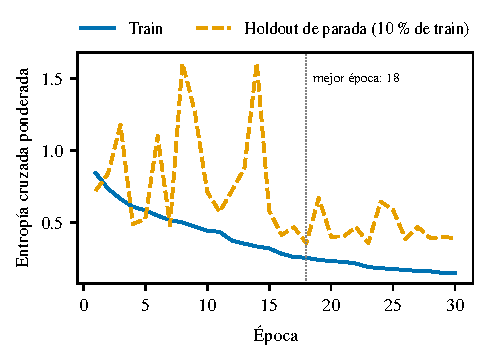
\includegraphics[width=\columnwidth]{figuras/perdida_cnn.pdf}
\caption{Pérdida de la CNN por época. La parada temprana usa un holdout del 10\,\% de los grupos de \emph{train}, no la validación.}
\label{fig:perdida}
\end{figure}

\emph{Por qué la prueba baja frente a la validación (0,76 $\to$ 0,60).} La caída es casi toda de \cls{regular} en AgriFreshNET: el RF llama \cls{bad} a 570 de sus 786 \cls{regular} de prueba, con tasas entre 87\,\% y 93\,\% en banano, pepino, berenjena y piña, pero menores al 10\,\% en tomate y melón amargo. Casi todos los productos de AgriFreshNET tienen solo de 2 a 5 lotes semanales de \cls{regular}, y cada lote va entero a una partición: a la validación le tocaron lotes que el RF generaliza bien y a la prueba lotes cuyo \cls{regular} se parece al \cls{bad} de otros lotes. Con tan pocas unidades independientes, la cifra de validación tiene una varianza que el bootstrap por grupos solo capta en parte (sus intervalos casi no se solapan). Por eso la cifra que sostenemos es la de prueba. No es un error de la partición: es el precio de medir sin fuga con pocos lotes.

\emph{Confusión entre fuente y clase.} En el segundo reparto, un RF que predice la \emph{fuente} con los mismos 359 atributos acertaba el 97,6\,\% (exactitud balanceada), y al entrenar en una fuente y evaluar en la otra el AUC buena-vs-mala caía de 0,98 a 0,72. Esto no prueba que el clasificador use la fuente como atajo, pero sí que lo aprendido en un dominio transfiere mal a otro. Agregar AFruitDB ayudó a que \cls{regular} no viniera de una sola fuente (en validación, el RF reconoce el 80\,\% de las \cls{regular} de AFruitDB).

\emph{Qué muestra el celular.} El fallo en guayaba, limón y mango no es de segmentación (los recortes se revisaron a mano): los limones y guayabas locales, amarillo-verdosos, se confunden con naranja, y el mango con papaya. Es un cambio de dominio. Banano y manzana, que tenían fotos de celular en \emph{train}, se reconocen casi siempre. En estado, el modelo acierta casi todas las buenas pero no detecta \cls{regular}. Con solo 4 piezas malas, el recall de \cls{bad} en celular no permite ninguna conclusión.

\emph{Comparación con la literatura.} Los artículos de FruitNet~\cite{meshram2022} y AFruitDB~\cite{mojumdar2025} describen conjuntos de datos; sus cifras no son comparables con las nuestras porque no usan la misma combinación de fuentes ni una partición por grupos de captura. Nuestra propia medición muestra por qué la comparación directa sería engañosa: partir por foto en lugar de por ráfaga inflaba el F1 de Kaggle unos 3,5 puntos, el mismo fenómeno de fuga que documentan Kapoor y Narayanan~\cite{kapoor2023}.

\emph{Qué funciona y qué no.} Funciona: separar la fruta del fondo, distinguir buena de mala cuando la captura se parece a la del entrenamiento, reconocer los productos vistos en celular y rechazar fotos inválidas. Falla: \cls{regular} entre lotes y fuentes, y frutas locales nunca vistas en fotos de celular.

\section{Ética e impactos}

La Tabla~\ref{tab:etica} relaciona cada decisión con los principios del Código de Ética del IEEE~\cite{ieee_ethics}: bienestar y privacidad del público (I.1), comunicar con honestidad capacidades e implicaciones (I.2 e I.5), dar crédito a terceros (I.5) y tratar con justicia a todas las personas (II.7).

La Tabla~\ref{tab:impactos} contrasta los impactos con lo que los resultados permiten afirmar. Ningún beneficio operativo (tiempo, desperdicio) está medido: requeriría una prueba de uso en campo.

\begin{table}[t]
\caption{Decisiones éticas y medidas adoptadas}
\label{tab:etica}
\centering
\scriptsize
\setlength{\tabcolsep}{3pt}
\begin{tabular}{@{}>{\raggedright\arraybackslash}p{0.24\columnwidth}>{\raggedright\arraybackslash}p{0.17\columnwidth}>{\raggedright\arraybackslash}p{0.53\columnwidth}@{}}
\toprule
Situación & Principio & Medida adoptada\\
\midrule
Fotos tomadas en casas, mercados o con la cámara de la app & I.1 privacidad & Encuadre solo de la pieza; la app procesa en memoria y no guarda imágenes; las fotos de celular no se redistribuyen.\\
Fotos aportadas por compañeros del curso & I.1 privacidad y consentimiento & Se usan solo las de la carpeta del curso, aportadas para este fin; no se redistribuyen, no aparecen personas y no se conservan metadatos.\\
Pieza mala predicha como buena & I.1 bienestar & Modelo final elegido por el menor número de errores \mb; se reporta el error; la app pide revisión si la confianza es baja o, cuando se activa la CNN, si RF y CNN discrepan.\\
Sesgo de los datos (frutas de India y Bangladesh) & II.7 trato justo; I.5 honestidad & Métricas por fuente y por fruta; se publica que las variedades locales fallan (Tabla~\ref{tab:celular}); la app no se ofrece para productos no vistos.\\
Fuentes con criterios distintos & I.5 honestidad & Mapeo de clases documentado; métricas por fuente; prueba externa con celular publicada aunque sea desfavorable.\\
Estado confundido con inocuidad & I.2 comunicar límites & La app dice que evalúa apariencia externa, no inocuidad ni interior, y que el tamaño es relativo.\\
Datos y código de terceros & I.5 crédito & Autores, licencias y cambios realizados (CC BY 4.0) en README e informe.\\
Etiquetado del conjunto externo & I.5 rigor & Etiquetas a ciegas, sin ver la app; validación y prueba se usan una vez, con candado.\\
\bottomrule
\end{tabular}
\end{table}

\begin{table}[t]
\caption{Matriz de impactos, evidencia y mitigación}
\label{tab:impactos}
\centering
\scriptsize
\setlength{\tabcolsep}{3pt}
\begin{tabular}{@{}>{\raggedright\arraybackslash}p{0.15\columnwidth}>{\raggedright\arraybackslash}p{0.44\columnwidth}>{\raggedright\arraybackslash}p{0.35\columnwidth}@{}}
\toprule
Dimensión & Impacto y evidencia & Mitigación\\
\midrule
Social & (+) Opinión consistente para una primera revisión. ($-$) 2,7\,\% de las malas pasan como buenas en prueba; \cls{regular} casi no se detecta. & Herramienta de apoyo, nunca decisión automática; revisión humana obligatoria en casos dudosos.\\
Económica & (+) Bajo costo: corre en un computador sin GPU y el RF no necesita TensorFlow. ($-$) Errores y recapturas cuestan; el ahorro no está medido. & Medir tiempo y tasa de reintento en una prueba de uso antes de afirmar ahorro.\\
Ambiental & (+) Una clasificación más informada podría evitar descartes. ($-$) Entrenar la CNN tomó $\approx$1\,h de CPU; el RF, minutos. & Preferir el RF (modelo final) y reentrenar solo con datos nuevos; registrar tiempos.\\
Global & ($-$) Con fotos de celular locales, el producto se acierta en 31,8\,\%: variedades y cámaras cambian por región. & No extender el uso a otros productos o regiones sin fotos locales en el entrenamiento y una nueva evaluación.\\
\bottomrule
\end{tabular}
\end{table}

\section{Conclusiones y trabajo futuro}

Construimos un sistema reproducible que identifica 13 productos, clasifica su apariencia externa en tres estados y estima su tamaño relativo, con una app que rechaza las fotos que no puede analizar. Aprendimos cuatro lecciones técnicas. (1) \emph{La unidad estadística es el grupo, no la foto}: definir mal el grupo produjo una fuga medible aunque las particiones fueran disjuntas, y el tamaño efectivo de validación es de 129 grupos, no de 3605 fotos. (2) \emph{La formulación con costo asimétrico decide el modelo}: con F1 empatado, el RF comete la mitad de errores \mb{} que el ensamble, y lo sigue haciendo en prueba. (3) \emph{El diagnóstico sesgo--varianza guió los experimentos}: explica por qué aumentar la capacidad de la CNN ayudó y por qué los giros empeoraron. (4) \emph{Fuente, lote y dominio pesan más que el modelo}: la caída a 0,596 en prueba viene de lotes de \cls{regular} y la prueba con celular muestra que el sistema solo es confiable con productos vistos en condiciones parecidas.

Como trabajo futuro, con sustento en los resultados: (i) fotos de celular de \emph{todas} las frutas en la mitad de entrenamiento, con al menos 40 piezas por clase para estimar recalls con semiancho de 0,15; (ii) más lotes independientes de \cls{regular} por producto; (iii) calibrar las probabilidades (por ejemplo, con \emph{temperature scaling}) antes de combinar RF y CNN; (iv) regularizar la CNN eligiendo con validación cruzada agrupada; y (v) medir el tamaño en milímetros con un objeto de referencia, $\hat D=D_{\text{ref}}\,d/d_{\text{ref}}$.

\begin{thebibliography}{18}

\bibitem{chapman2000}
P.~Chapman \emph{et al.}, ``CRISP-DM 1.0: Step-by-step data mining guide,'' SPSS Inc., 2000.

\bibitem{otsu1979}
N.~Otsu, ``A threshold selection method from gray-level histograms,'' \emph{IEEE Trans. Syst., Man, Cybern.}, vol.~9, no.~1, pp.~62--66, 1979.

\bibitem{rother2004}
C.~Rother, V.~Kolmogorov, and A.~Blake, ``GrabCut: Interactive foreground extraction using iterated graph cuts,'' \emph{ACM Trans. Graph.}, vol.~23, no.~3, pp.~309--314, 2004.

\bibitem{ojala2002}
T.~Ojala, M.~Pietikäinen, and T.~Mäenpää, ``Multiresolution gray-scale and rotation invariant texture classification with local binary patterns,'' \emph{IEEE Trans. Pattern Anal. Mach. Intell.}, vol.~24, no.~7, pp.~971--987, 2002.

\bibitem{cortes1995}
C.~Cortes and V.~Vapnik, ``Support-vector networks,'' \emph{Mach. Learn.}, vol.~20, pp.~273--297, 1995.

\bibitem{breiman2001}
L.~Breiman, ``Random forests,'' \emph{Mach. Learn.}, vol.~45, pp.~5--32, 2001.

\bibitem{ioffe2015}
S.~Ioffe and C.~Szegedy, ``Batch normalization: Accelerating deep network training by reducing internal covariate shift,'' in \emph{Proc. ICML}, 2015, pp.~448--456.

\bibitem{kingma2015}
D.~P. Kingma and J.~Ba, ``Adam: A method for stochastic optimization,'' in \emph{Proc. ICLR}, 2015.

\bibitem{efron1993}
B.~Efron and R.~J. Tibshirani, \emph{An Introduction to the Bootstrap}. New York, NY, USA: Chapman \& Hall, 1993.

\bibitem{pedregosa2011}
F.~Pedregosa \emph{et al.}, ``Scikit-learn: Machine learning in Python,'' \emph{J. Mach. Learn. Res.}, vol.~12, pp.~2825--2830, 2011.

\bibitem{kapoor2023}
S.~Kapoor and A.~Narayanan, ``Leakage and the reproducibility crisis in machine-learning-based science,'' \emph{Patterns}, vol.~4, no.~9, Art. no.~100804, 2023.

\bibitem{meshram2022}
V.~Meshram and K.~Patil, ``FruitNet: Indian fruits image dataset with quality for machine learning applications,'' \emph{Data Brief}, vol.~40, Art. no.~107686, 2022, doi: 10.1016/j.dib.2021.107686.

\bibitem{park_kaggle}
R.~Park, ``Fruit Quality Classification,'' Kaggle. [Online]. Available: \url{https://www.kaggle.com/datasets/ryandpark/fruit-quality-classification}

\bibitem{risdin2026}
F.~Risdin, H.~Salauddin, T.~A. Tufa, and M.~J. Hossain, ``AgriFreshNET freshness and shelf-life image dataset,'' Mendeley Data, v1, 2026, doi: 10.17632/42m5tb7yv9.1.

\bibitem{mojumdar2025}
M.~U. Mojumdar, S.~Islam, M.~A. Mamun, R.~Hasan, S.~M.~T. Siddiquee, and N.~R. Chakraborty, ``AFruitDB: A comprehensive dataset of six commonly used Asian fruits for advanced grading and biodiversity insights,'' \emph{Data Brief}, vol.~59, Art. no.~111380, 2025, doi: 10.1016/j.dib.2025.111380.

\bibitem{mojumdar2024data}
M.~U. Mojumdar, M.~A. Mamun, S.~Islam, and R.~Hasan, ``A dataset of common Asian fruits for quality grading and biodiversity research,'' Mendeley Data, v1, 2024, doi: 10.17632/bz65dz2pbj.1.

\bibitem{apo3_fotos}
Estudiantes de Algoritmos y Programación III, ``Photos of Fruits and Vegetables | APO III,'' carpeta compartida del curso, Universidad Icesi, 2026.

\bibitem{ieee_ethics}
IEEE, ``IEEE Code of Ethics,'' 2020. [Online]. Available: \url{https://www.ieee.org/about/corporate/governance/p7-8.html}

\end{thebibliography}

\end{document}
